\section{Results and Analysis}\label{sec:results}

% NOTE: All measured values in this section are \phX placeholders pending the
% training rerun (fixed SH17 remap + gas-mask class). Drop numbers in from the
% rerun log; do not reuse figures from the earlier fusion run.

The fused-dataset YOLOv8n detector reaches \phX\% precision, \phX\% recall, and \phX\% mAP@50 across all classes while processing a frame in \phX~ms on a Tesla T4-class GPU. That combination is the central finding of this section: accuracy sufficient for operational alerting, delivered at a speed and model footprint that fit the retrofit deployment model on existing CCTV infrastructure. Sections~\ref{sec:results-training} and~\ref{sec:results-perclass} report the detector's aggregate and per-class behavior, Section~\ref{sec:results-ocp} scopes the in-progress site-specific fine-tuning stage, Section~\ref{sec:results-cases} presents qualitative case studies of the LLM judge, Section~\ref{sec:results-errors} analyzes error structure, and Section~\ref{sec:results-runtime} quantifies runtime feasibility.

\subsection{Training Performance}\label{sec:results-training}

\begin{figure}[t]
\centering
% TODO: regenerate from rerun (fixed SH17 remap + gas-mask class); current file is from the superseded fusion run
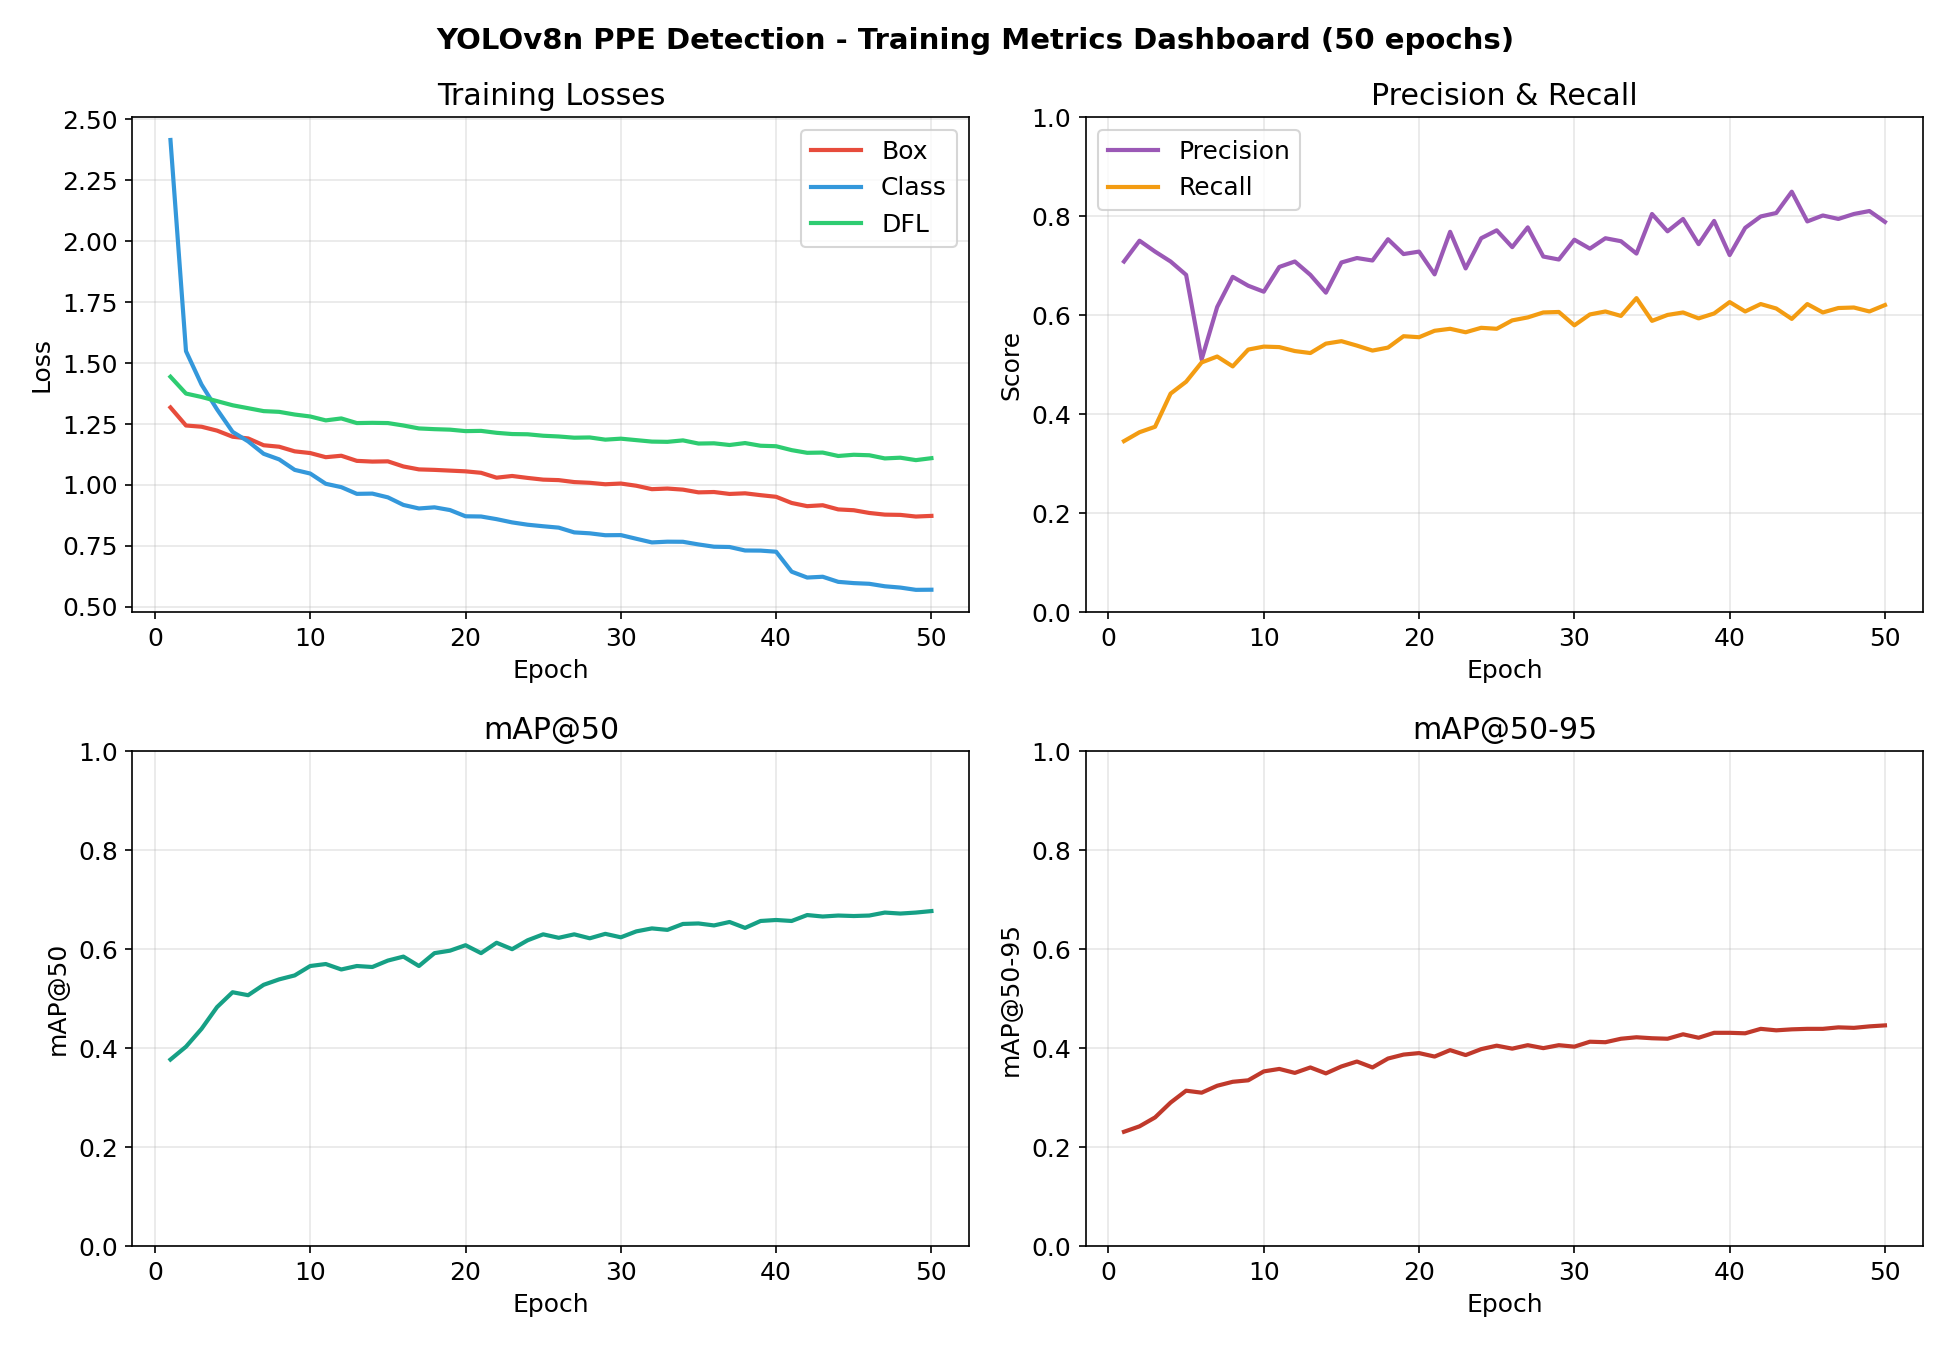
\includegraphics[width=\columnwidth]{figures/dashboard.png}
\caption{Training dashboard for the fused-dataset run: box, classification, and DFL loss curves (train and validation) with precision, recall, mAP@50, and mAP@50--95 per epoch.}
\label{fig:dashboard}
\end{figure}

Figure~\ref{fig:dashboard} summarizes the \phX-epoch training run at $640\times640$ input resolution with batch size 16. Box, classification, and distribution focal (DFL) losses decline from \phX, \phX, and \phX at the first epoch to \phX, \phX, and \phX at the final epoch, with validation losses tracking the training curves throughout. Precision and recall stabilize after approximately \phX epochs at \phX\% and \phX\% respectively. The final model attains \phX\% mAP@50 and \phX\% mAP@50--95 on the validation split. All headline values are taken from the best checkpoint (\texttt{best.pt}), selected on validation mAP@50--95. Unless noted otherwise, reported metrics use the \phX split of the fused dataset; the same split is used consistently across Table~\ref{tab:perclass} and the error analysis of Section~\ref{sec:results-errors}.
% TODO: decide val split vs. held-out test split for headline tables (structure.md open item); a held-out test set is the stronger claim.

\subsection{Detection Performance by Class}\label{sec:results-perclass}

Table~\ref{tab:perclass} breaks performance down by class. The fused dataset inherits markedly uneven per-class support from its source corpora \cite{roboflowppe, ahmad2024sh17}: person, helmet, and vest instances dominate, while negative-state classes (no\_helmet, no\_gloves, no\_goggle) and the gas-mask class introduced by this work's augmentation have far fewer validation instances. Rows for low-support classes should therefore be read alongside the support caveats in Section~\ref{sec:results-errors}, where the imbalance and its consequences are examined directly.

\begin{table}[t]
\caption{Per-class detection performance on the validation split. All values pending training rerun.}
\label{tab:perclass}
\centering
\begin{tabular}{lccc}
\toprule
Class & Precision (\%) & Recall (\%) & mAP@50 (\%) \\
\midrule
Person      & \phX & \phX & \phX \\
helmet      & \phX & \phX & \phX \\
no\_helmet  & \phX & \phX & \phX \\
vest        & \phX & \phX & \phX \\
gloves      & \phX & \phX & \phX \\
no\_gloves  & \phX & \phX & \phX \\
goggles     & \phX & \phX & \phX \\
no\_goggle  & \phX & \phX & \phX \\
boots       & \phX & \phX & \phX \\
gas mask    & \phX & \phX & \phX \\
\midrule
\textbf{All classes} & \phX & \phX & \phX \\
\bottomrule
\end{tabular}
\end{table}

\subsection{Effect of Site-Specific Fine-Tuning}\label{sec:results-ocp}

The OCP fine-tuning stage is in progress at the time of writing; no site-specific results are claimed here. The planned evaluation compares the generic fused-dataset model against the OCP-weighted model on an identical held-out set of site imagery, reporting per-class deltas and side-by-side qualitative detections under the dust, lighting, and uniform conditions that motivate the domain-adaptation stage. Figure~\ref{fig:ocp-compare} reserves the position for this comparison, pending completion of the fine-tuning run and clearance of site imagery for publication.

\begin{figure}[t]
\centering
\fbox{\parbox[c][4cm][c]{0.9\columnwidth}{\centering Placeholder: side-by-side detections,\\generic fused-dataset model vs.\ OCP-weighted model,\\on identical OCP site imagery.}}
\caption{Generic vs.\ OCP-weighted model on identical site imagery. TODO: pending OCP fine-tuning run and imagery clearance.}
\label{fig:ocp-compare}
\end{figure}

\subsection{LLM Judge Qualitative Case Studies}\label{sec:results-cases}

The judge stage is evaluated qualitatively. The protocol selects three to five real flagged detections from pilot footage and, for each, presents the detection crop, the verbatim \texttt{reason} field returned by the Qwen2.5-VL judge \cite{qwen25vl}, and the final verdict. The case set is chosen to include at least one false positive that the judge correctly rejects (for example, a glare or occlusion artifact of the kind that drives false-alarm load in manual CCTV monitoring \cite{donald2015}) and at least one genuine violation that the judge confirms, so that both failure-suppression and violation-preservation behavior are visible on real inputs. Table~\ref{tab:cases} holds the case scaffold.

We state explicitly: no quantitative false-positive-reduction figure is claimed for the judge stage anywhere in this paper. The case studies demonstrate the mechanism operating on real detections; they do not measure its aggregate effect. Quantitative benchmarking of the judge, over a labeled alert set with a confirm/reject confusion matrix, is future work (Section~\ref{sec:discussion}).

\begin{table*}[t]
\caption{LLM judge case studies: flagged detections with verbatim judge output. TODO: fill from pilot judge runs; include detection crops as an accompanying figure once imagery is cleared.}
\label{tab:cases}
\centering
\begin{tabular}{clcp{8.5cm}}
\toprule
Case & Flagged class & Judge verdict & Judge reason (verbatim) \\
\midrule
1 & TODO & TODO & TODO \\
2 & TODO & TODO & TODO \\
3 & TODO & TODO & TODO \\
4 & TODO & TODO & TODO \\
5 & TODO & TODO & TODO \\
\bottomrule
\end{tabular}
\end{table*}

\subsection{Error Analysis}\label{sec:results-errors}

Confusion concentrates among visually similar class pairs. The equipment/absence pairs (helmet vs.\ no\_helmet, goggles vs.\ no\_goggle) are separated by fine-grained head-region cues that degrade with distance and partial occlusion; \phX\% of no\_helmet errors fall into this pattern. Dark headwear and hoods account for a further \phX\% of helmet-related confusions, and gloves at long range are confused with bare hands in \phX\% of cases.

Class support shapes these figures. The helmet class holds \phX validation instances against \phX for no\_helmet, so the two rows in Table~\ref{tab:perclass} rest on very different evidence bases, and the same asymmetry applies to the other equipment/absence pairs. Boots, no\_goggle, and gas mask each fall below \phX validation instances; their per-class metrics carry wide uncertainty and are treated as indicative rather than conclusive. How much of the observed error structure stems from the multi-source fusion itself, from the nano-scale model capacity, or from support imbalance is a question the per-class numbers will settle once the rerun completes.
% TODO: after rerun, decide framing per [OPEN: results_posture] in chapter-plan.md (own weak classes openly vs. relax the caveats).

\subsection{Runtime and Deployment Feasibility}\label{sec:results-runtime}

Single-frame latency on a Tesla T4-class GPU is \phX~ms end to end: \phX~ms preprocessing, \phX~ms inference, and \phX~ms postprocessing at $640\times640$ resolution. At an analysis rate of \phX frames per second per camera, one GPU of this class sustains approximately \phX concurrent camera feeds, before any batching across streams.

The model itself is small: YOLOv8n comprises 3.0M parameters at 8.1 GFLOPs, with a 6.3~MB weight file \cite{ultralytics2023}, in line with edge-oriented PPE deployments \cite{edgeyolo2024}. Together these figures support the retrofit argument. A site's existing cameras keep their role as passive sensors; the entire detection workload for a multi-camera installation concentrates on a single commodity GPU server attached to the existing network, with no per-camera hardware and no replacement of the installed CCTV base. The judge stage adds latency only on the flagged-detection path, which is orders of magnitude sparser than the frame stream itself, so detector throughput governs feed capacity.
